\section{Loi d’une variable aléatoire réelle - Fonction de répartition}

\subsection{Variable aléatoire réelle et sa loi}

$\mathbb{R}$ sera toujours muni de sa tribu borélienne $\mathscr{B}(\mathbb{R})$.

\theoremstyle{rappel}
\begin{rappel}
    Pour tout $a\in \mathbb{R}$, on a $]-\infty,a]\in \mathscr{B}(\mathbb{R})$.
\end{rappel}
\theoremstyle{definition}
\begin{definition}
    Une \textbf{variable aléatoire réelle} $X: (\Omega,\mathscr{A})\to (\mathbb{R},\mathscr{B}(\mathbb{R}))$ est telle que
    pour tout $B\in\mathscr{B}(\mathbb{R})$, on a $X^{-1}(B)=\{X\in B\}\in\mathscr{A}$.\\
\textcolor{blue}{$X$ est une application mesurable de $(\Omega,\mathscr{A})$ dans $(\mathbb{R},\mathscr{B}(\mathbb{R}))$}.
\end{definition}
On pose: $$\mathbb{P}_X(B) = \mathbb{P}(X \in B).$$
\textcolor{red}{Alors la loi $P_X$ de $X$ est une probabilité sur (\mathbb{R},\mathscr{B}(\mathbb{R}))}.\\
\textbf{Question}: Comment caractériser $\mathbb{P}_X$ ?\\
\textbf{Grosse difficulté}: $\mathbb{R}$ est constitué d’une infinité \textbf{non dénombrable} de  singletons.

\subsection{Fonction de répartition}
\theoremstyle{definition}
\begin{definition}
    On appelle \textbf{fonction de répartition} de $X$ la fonction suivante:
\textcolor{blue}{$$F_X(x)=\mathbb{P}_X(]-\infty,x])=\mathbb{P}(X\leq x) \mbox{   } \forall x\in\mathbb{R}. $$}
\end{definition}

\theoremstyle{proposition}
\begin{proposition}
La fonction de répartition $F_X$ caractérise la probabilité $\mathbb{P}_X$ et elle vérifie
les trois conditions suivantes:

\begin{enumerate}
\item \textcolor{blue}{elle est croissante}\label{prop:prop1.1}
\item \textcolor{blue}{elle est continue à droite}\label{prop:prop1.2}
\item \textcolor{blue}{$\liminf\limits_{x\rightarrow-\infty}F_X(x)=0$ ,
$\limsup\limits_{x\rightarrow+\infty}F_X(x)=1$}\label{prop:prop1.3}
\end{enumerate}
\end{proposition}

\begin{corollary}
\textcolor{blue}{Si deux variables aléatoires ont la même fonction de répartition, alors
elles ont la même loi.}
\end{corollary}
Ce corollaire est un résultat d’unicité.

\theoremstyle{theorem}
\begin{theorem}
\textcolor{blue}{Si F vérifie les conditions (\ref{prop:prop1.1})–(\ref{prop:prop1.3}) ci-dessus, c’est la fonction de
répartition d’une (unique) probabilité sur $(\mathbb{R},\mathscr{B}(\mathbb{R}))$}. (Admis).
\end{theorem}
Ce théorème est un résultat d’existence. Il existe une probabilité $\mu$ sur $(\mathbb{R},\mathscr{B}(\mathbb{R}))$
telle que pour tout $x\in\mathbb(R)$, $$F(x)=\mu(]-\infty,x]).$$
C’est un théorème de construction de mesure qui est très délicat à
montrer.\\
\textcolor{blue}{On ne peut pas en général définir cette probabilité sur la tribu $\mathcal{P}(\mathbb{R})$
des parties de $\mathbb{R}$}.\\
\textcolor{blue}{Comme $F_X$ est croissante, elle admet une limite à gauche en chaque point, notée $F_X(x-)$, et
$F_X(x-)=\mathbb{P}(X<x)=\mathbb{P}_X(]-\infty,x])$}.

\begin{align}
\mathbb{P}_X(]x,y]) &= \mathbb{P}(x<X\leq y) = F_X(y)-F_X(x),\\
\mathbb{P}_X([x,y]) &= \mathbb{P}(x\leq X\leq y) = F_X(y)-F_X(x-).
\end{align}

En particulier, \textcolor{red}{ $ \mathbb{P}_X(\{x\})=F_X(x)-F_X(x-)$} est le saut de la fonction $F_X$ au point $x$. On a donc

\begin{proposition}
\textcolor{blue}{$$\mathbb{P}_X(\{x\})=\mathbb{P}(X=x)=0 \iff F_X \text{ est continue en } x.$$}
\end{proposition}

\begin{example}
\textcolor{blue}{$F(x)=x$ sur $[0,1]$, avec $F(x)=0$ pour $x\leq0$ et $F(x)=1$ pour $x\geq1$} détermine une probabilité
appelée \textbf{probabilité uniforme sur} $[0,1]$ ou encore \textbf{mesure de Lebesgue sur} $[0,1]$, qui correspond à
"la longueur" des intervalles.
\end{example}

\begin{remark}
Si $X$ prend un nombre fini de
valeurs, sa fonction de répartition
est une fonction en escalier.
\begin{figure}[h]
\centering
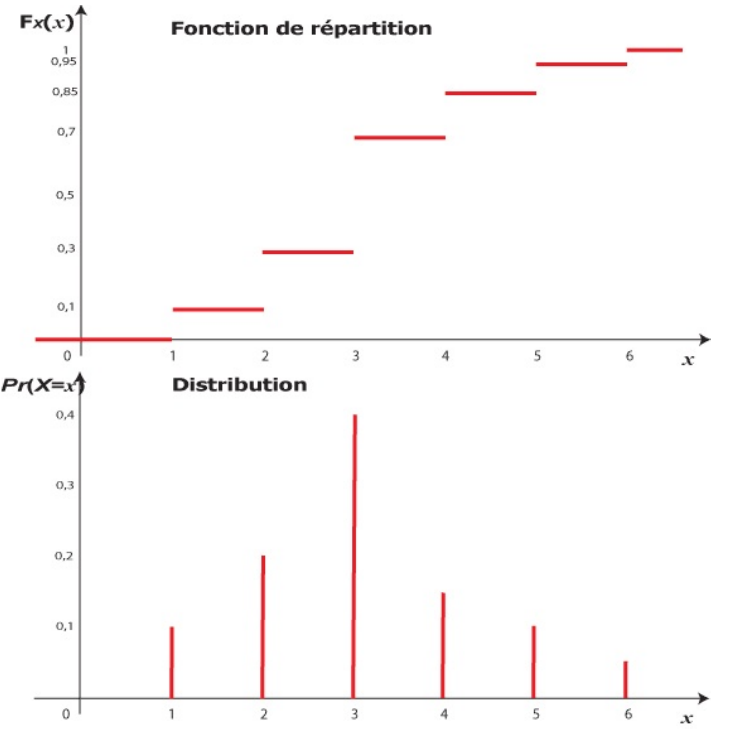
\includegraphics[width=8cm]{content/figureremarque1.PNG}
\end{figure}
%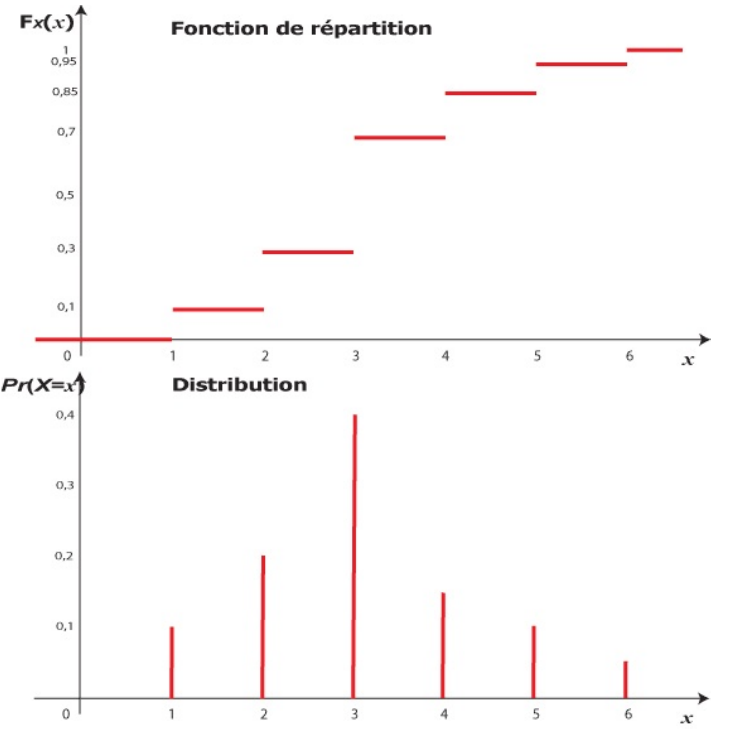
\includegraphics{content/figureremarque1.PNG}
\end{remark}






































\iffalse
\section{Loi d’une variable aléatoire réelle - Fonction de répartition}\label{chap:1}

% This is a comment
Ici, nous discutons des concepts nécessaires pour tirer des conclusions statistiques à partir d'un échantillon de
données sur une population d'intérêt. Par exemple, supposons que nous connaissions le salaire de départ d'un
échantillon de 100 étudiants diplômés en droit. Nous pouvons utiliser ces connaissances pour tirer des conclusions
sur le salaire prévu pour la population de tous les étudiants diplômés en droit. De même, si un médicament nouvellement
développé est administré à un échantillon de patients tuberculeux sélectionnés, alors certains patients peuvent montrer
une amélioration et d'autres non, mais nous nous intéressons aux conséquences pour l'ensemble de la population de
patients. Dans la suite de ce chapitre, nous décrivons les concepts théoriques nécessaires pour tirer de telles
conclusions. Ils constituent la base des tests statistiques et de l'inférence.


\subsection{Variables aléatoires}
Les variables aléatoires nous aident à voir les données collectées comme le résultat d'une expérience aléatoire.
Considérez l'expérience simple de lancer une pièce. Si une pièce est lancée, alors on peut observer soit «face» (F)
ou «pile» (P). L'apparition de «face» ou de «pile» est aléatoire, et le résultat exact ne sera connu qu'après avoir
lancé la pièce. Nous pouvons lancer la pièce plusieurs fois et obtenir une séquence de sorties. Par exemple, si une
pièce est lancée sept fois, puis l'un des résultats peut être F, F, P, F, P, P, P. Ce résultat est la conséquence
d'une expérience aléatoire, et il peut être utile de distiller la séquence des résultats en nombres significatifs.
Une option consiste à les résumer par une variable $X$, qui prend les valeurs $x_1 = 1$ (pour pile) et $x_2 = 0$
(pour face). Cela peut être décrit dans le cadre d'une expérience aléatoire où $\Omega= \{\omega_1, \omega_2\}$ avec les événements
$A_1 = \{\omega_1\} = 1 = \text{pile}$ et $A_2 = \{\omega_2\} = 0 = \text{face}$.\\

La variable aléatoire $X$ est désormais associée à des nombres réels et, par conséquent, elle décrit le résultat possible
de toute expérience de lancer de pièces. Les résultats observés F, F, P, F, P, P, P se rapportent à un échantillon
spécifique, une réalisation unique de cette expérience. On peut écrire $X(\omega_1) = 1$ et $X(\omega_2) = 0$ avec
$\omega_1, \omega_2 \in \Omega$
et $1,0 \in \mathcal{R}$ où $\mathcal{R}$ est l'ensemble des nombres réels. Nous savons que dans toute expérience de lancer de pièces, la
probabilité que face soit observée est $P (X (\omega_1) = 1) = 0,5$ et que pile observée est
$P (X (\omega_2) = 0) = 0,5$. Nous pouvons donc considérer $X$ comme une variable aléatoire qui recueille les
résultats possibles d'une expérience aléatoire et capture l'incertitude qui leur est associée.

\begin{table}[h!]
    \centering
    \caption{Exemples de variables aléatoires}
    \begin{tabular}{||c | c | c ||}
        \hline
        $X$ & Événement  & Réalisations de $X$\\ [0.5ex]
        \hline\hline
        Lancer d'un dé & $A_i$: nombre $i$ ($i = 1, 2,\dots, 6$) & $x = i$ \\\hline
        Durée de d'une TV & $A_i$: temps de survie est $i$ mois $(i = 1, 2, \dots)$ & $x = i$  \\\hline
        Roulette (Jeu de hasard) &\makecell{  $A_1$: rouge\\ $A_2$: noir\\\ $A_3$: vert (zéro)} &\makecell{ $x_1=1$\\$x_2=2$\\ $x_3=0$} \\ [1ex]
        %info & \makecell{ line1 \\\hline line2 }  &  blubb&\\
        \hline
    \end{tabular}

    \label{table:1}
\end{table}

\theoremstyle{definition}
\begin{definition}{}
Soit $\omega$ représente l'espace échantillon d'une expérience aléatoire, et soit $\mathcal{R}$ l'ensemble des nombres
réels. Une variable aléatoire est une fonction $X$ qui attribue à chaque élément $\omega \in \Omega$ un et un seul
nombre $X (\omega) = x, x \in \mathcal{R}$, c'est-à-dire.
\begin{equation}
    X : \Omega \to \mathcal{R}
\end{equation}
\end{definition}

\begin{example}
    Les caractéristiques d'une expérience de jet de dé, d'un jeu de roulette ou de la durée de vie d'un téléviseur
    peuvent toutes être décrites par une variable aléatoire, voir Tableau \ref{table:1}. Les événements impliquent un
    caractère aléatoire, et si nous avons des connaissances sur le processus aléatoire, nous pouvons attribuer des
    probabilités $P (X = x_i)$ à chaque événement, par ex. lors du lancer d'un dé, la probabilité d'obtenir
    un «$1$» est $P (X = 1) = 1/6$ et la probabilité d'obtenir un «$2$» est $P (X = 2) = 1/6$.
\end{example}
Plus généralement, on peut dire qu'il est obligatoire de connaître $ P (X \in A) $ pour tous les $ A $ possibles qui sont
des sous-ensembles de $ \ mathcal {R} $. Si nous choisissons $ A = (-\infty, x], x ∈ \ mathcal {R} $, nous avons
$$ P(X\in A) = P(X\in (-\infty,x])=P(-\infty<X\leq x)=P(x\leq x). $$
Cette considération donne lieu à la définition de la Fonction de répartition.

\subsection{Fonction de répartition}
\theoremstyle{definition}
\begin{definition}{}\label{def:foncrep}

La fonction de répartition (\textbf{cumulative distribution function}) d'une variable aléatoire X est définie comme

\begin{equation}
    F(x) = P(X\leq x).
\end{equation}
\end{definition}
Nous pouvons voir que la fonction de répartition est utile pour obtenir les probabilités liées à l'occurrence d'événements
aléatoires. Notons que la Fonction de répartition empirique\footnote{La fonction de répartition empirique $ F (x) $ est
définie comme:
\begin{equation}
    F(x) = \sum_{a_j\leq x}f(a_j)
\end{equation}
avec $f_j =n_j/n$, $n$ le nombre d'observation.\\ Cette définition implique que F (x) est une fonction monotone non
décroissante, $0\leq F(x)\leq1$, $\lim_{x \to-\infty}F(x) = 0$, $\lim_{x \to+\infty}F(x) = 1$, et F(x) est continue à
droite.} et la Fonction de répartition sont étroitement liées et ont donc une définition et des règles de calcul
similaires.\\

La Définition \ref{def:foncrep} applique les propriétés suivantes de la fonction de répartition:
\begin{itemize}
\item $F(x)$ est une fonction monotone non décroissante (si $x_1\leq x_2$, alors $F(x_1)\leq F(x_2)$),
\item $\lim_{x\to-\infty}F(x)=0$ (la limite inf de $F$ est $0$),
\item $\lim_{x\to+\infty}F(x)=1$ (la limite sup de $F$ est $1$),
\item $F(x)$ est continue à droite, et
\item $0\leq F(x)\leq1$ pour tout $x\in\mathcal{R}$.
\end{itemize}
Une autre notation pour $F(x)=P(X\leq x)$ est $F_{X}(x)$, mais on utilisera $F(x)$

\subsubsection{La fonction de répartition des variables aléatoires continues}
Avant de donner quelques exemples sur la signification et l'interprétation de la fonction de répartition, nous devons
d'abord considérer quelques définitions et théorèmes.

\theoremstyle{definition}
\begin{definition}{}\label{def:vacont}
Une variable aléatoire $ X $ est dite \textbf{continue} s'il y a une fonction
$ f (x) $ tel que pour tout $ x \in \mathcal {R} $
\begin{equation}
F(x) = \int_{-\infty}^{x}f(t)d(t)
\end{equation}
existe. $F(x)$ est la fonction de répartition de $X$, et $f(x)$  est la densité de probabilité de $x$ et
$\frac{d}{dx}F(x)=f(x)$ pour tous les $x$ qui sont des points de continuité de $f$.
\end{definition}
\theoremstyle{theorem}
\begin{theorem}{}\label{thm:1.1}
Pour qu'une fonction $ f (x) $ soit une fonction de densité de probabilité de $ X $, elle doit satisfaire aux
conditions suivantes:
\begin{enumerate}
\item $f(x)\geq0$ pour tout $x\in\mathcal{R}$
\item $\int_{-\infty}^{+\infty}f(x)dx=1$.
\end{enumerate}
\end{theorem}

\theoremstyle{theorem}
\begin{theorem}{}\label{thm:1.2}
Soit $ X $ une variable aléatoire avec une fonction de répartition $ F (x) $. Si $ x_1 <x_2 $,
où $ x_1 $ et $ x_2 $ sont des constantes connues,
$ P (x_1 \leq X \leq x_2) = F (x_2) - F (x_1) = \int_ {x_1} ^ {x_2} f (x) dx $.
\end{theorem}

\theoremstyle{theorem}
\begin{theorem}\label{thm:1.3}
La probabilité qu'une variable aléatoire continue prenne une valeur particulière $ x_0 $ est nulle:
\begin{equation}
P(X=x_0)=0.
\end{equation}
\end{theorem}
\begin{pruf}
Considérons un intervalle $(x_0-\delta,x_0]$ avec $\delta\geq0$. Il découle du Théorème \ref{thm:1.2} que
$P(x_0-\delta<X\leq x_0)=F(x_0)-F(x_0-\delta)$ et donc

\begin{align*}
P(X=x_0) & = \lim_{\delta\to0}P(x_0 -\delta<X\leq x_0)\\&= \lim_{\delta\to0}[F(x_0) - F(x_0 -\delta)]\\&= F(x_0) - F(x_0) =0.
\end{align*}
\end{pruf}

\begin{example}\label{exemple:1}
Prenons la variable aléatoire continue «temps d'attente pour le train». Supposons qu'un train arrive toutes les 20 min.
Par conséquent, le temps d'attente d'une personne particulière est aléatoire et peut être n'importe quel temps contenu
dans l'intervalle $ [0, 20] $. Nous pouvons commencer à décrire la fonction de densité de probabilité requise comme

$$f(n) = \begin{cases} k, & \mbox{pour   } 0\leq x\leq20 \\ 0, & \mbox{ailleurs } \end{cases}$$

où $k$ est une constante inconnue. Maintenant, en utilisant la condition (2) du Théorème \ref{thm:1.1}, on a
$$1=\int_0^{20}f(x)dx=[kx]_{0}^{20}=20k$$
qui doit être remplie. Cela donne $ k = 1/20 $ qui est toujours supérieur à 0, et par conséquent, la condition (1)
du Théorème \ref{thm:1.1} est également remplie. Il s'ensuit que

$$f(n) = \begin{cases} \frac{1}{20}, & \mbox{pour   } 0\leq x\leq20 \\ 0, & \mbox{ailleurs } \end{cases}$$

est la fonction de densité de probabilité décrivant le temps d'attente pour le train. Nous pouvons maintenant utiliser
Définition \ref{def:vacont} pour déterminer la fonction de répartition:
$$F(x)=\int_{0}^{x}f(t)dt=\int_{0}^{x}\frac{1}{20}dt=\frac{1}{20}[t]_{0}^{x}=\frac{1}{20}x.$$
Supposons que nous souhaitons calculer la probabilité d'un temps d'attente compris entre 15 $ et 20 $ min.
Cela peut être calculé en utilisant le Théorème \ref{thm:1.2}:
$$P(15\leq X\leq20)=F(20)-F(15)=\frac{20}{20}-\frac{15}{20}=0.25.$$
Nous pouvons également obtenir cette probabilité à partir du graphique de la fonction de répartition, voir Fig. \ref{fig:exemple1}
où la densité de probabilité et la fonction de répartition de cet exemple sont illustrées.\\

La définition d'une fonction, par exemple la fonction de répartition, est simple dans R: on peut utiliser
la commande \textit{function} suivie de la spécification des variables que la fonction évalue entre parenthèses
(par exemple $ x $) et la fonction elle-même entre accolades (par exemple $ x / 20 $ ). Les fonctions peuvent être
tracées à l'aide de la commande \textit{curve}:

\begin{verbatim}
cdf <- function(x){1/20*x}
curve(cdf,from=0,to=20)
\end{verbatim}


\begin{figure}%
\centering
\subfloat[Fonction de densité de probabilité]{{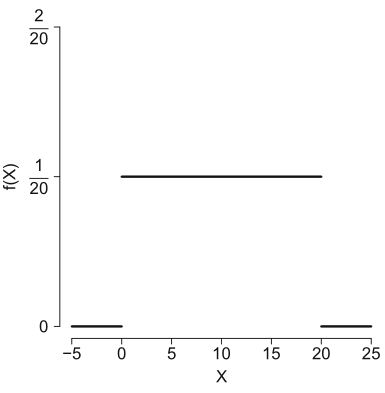
\includegraphics[width=5cm]{content/pdf.PNG} }}%
\qquad
\subfloat[Fonction de répartition]{{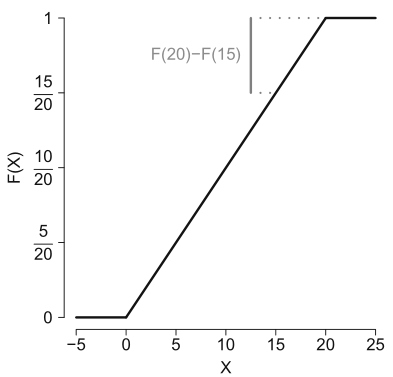
\includegraphics[width=5cm]{content/cdf.PNG} }}%
\caption{Fonction de densité de probabilité et fonction de répartition pour le temps d'attente dans l'exemple \ref{exemple:1}}%
\label{fig:exemple1}%
\end{figure}
\end{example}
\subsubsection{La fonction de répartition des variables aléatoires discrètes}

\theoremstyle{definition}
\begin{definition}
Une variable aléatoire $X$ est définie comme étant \textbf{discrète} si son espace de probabilité est fini ou dénombrable,
c'est-à-dire si elle ne prend qu'un nombre fini ou dénombrable de valeurs. Notez qu'un ensemble $V$ est censé
être \textbf{dénombrable}, si ses éléments peuvent être listés, c'est-à-dire qu'il existe une bijection entre $V$
et les entiers positifs.
\end{definition}

\begin{example}\label{exemple:2}
Prenons l'exemple du lancement d'une pièce où chaque essai donne lieu à face (F) ou à pile (P), chacune se produisant
avec la même probabilité $0,5$. Lorsque la pièce est lancée plusieurs fois, nous pouvons observer des séquences telles
que F, P, F, F, P, F, F, P et P, \dots. L'espace d'échantillon est $\Omega = \{F, P\}$. Soit la variable aléatoire $X$ le
nombre d'essais requis pour obtenir la troisième tête, puis $X = 4$ pour la séquence donnée ci-dessus.
Clairement, l'espace de $X$ est l'ensemble $(3,4,5, \dots)$. Nous pouvons voir que $X$ est une variable aléatoire
discrète car son espace est fini et peut être compté. Nous pouvons également attribuer certaines probabilités à
chacune de ces valeurs, par exemple $P (X = 3) = p_1$ et $P (X = 4) = p_2$.
\end{example}

\theoremstyle{definition}
\begin{definition}
Soit $X$ une variable aléatoire discrète qui prend $k$ valeurs différentes.
La \textbf{fonction de masse} de probabilité (probability mass function) de $X$ est donnée par
\begin{equation}\label{eq:foncmass}
f(X) = P(X = x_i)=p_i \text{ pour tout } i=1,2,\dots,k.
\end{equation}
Il est nécessaire que les probabilités $p_i$ remplissent les conditions suivantes:
\begin{enumerate}
\item $0\leq p_i\leq1$,
\item $\sum_{i=1}^{k}p_i=1$.
\end{enumerate}
\end{definition}

\theoremstyle{definition}
\begin{definition}
Étant donné (\ref{eq:foncmass}), nous pouvons écrire la fonction de répartition d'une variable aléatoire discrète comme
\begin{equation}\label{eq:frvd}
F(x)=\sum_{i=1}^{k} \mathds{1}_{\{x_i \leq x\}}p_i,
\end{equation}
où $\mathds{1}$ est une fonction indicatrice définie comme
$$\mathds{1}_{\{x_i \leq x\}} = \begin{cases} 1, & \mbox{si   } x_i\leq x\\ 0, & \mbox{ailleurs } \end{cases}$$
\end{definition}

La fonction de répartition d'une variable discrète est toujours une \textbf{fonction en escalier}.\\

Nous pouvons facilement calculer différents types de probabilités pour des variables aléatoires discrètes en utilisant
la fonction de répartition. Soit $ a $ et $ b $ des constantes connues, alors
\begin{align}\label{eq:freqs}
P(X\leq a) & = F(a),\label{sub-eq-1:8}\\P(X<a) &= P(X\leq a)-P(X=a)=F(a)-P(X=a),\\P(X>a) &= 1-P(X\leq a)=1-F(a),\\
P(X\geq a) &=1-P(X<a)=1-F(a)+P(X=a),\\ \nonumber P(a\leq X\leq b) &= P(X\leq b) - P(X<a)\\ &=F(b)-F(a)+P(X=a),\\
P(a<X\leq b) &= F(b)-F(a),\\P(a<X<b) &= F(b)-F(a)-P(X=b),\label{sub-eq-1:14}\\P(a\leq X<b)&=F(b)-F(a)-P(X=b)+P(X=a).\label{sub-eq-1:1}
\end{align}
\begin{remark}
Les équations (\ref{eq:frvd})-(\ref{sub-eq-1:1}) peuvent également être utilisées pour les variables continues, mais dans ce cas,
$P (X = a) = P (X = b) = 0$ (voir le Théorème \ref{thm:1.3}), et donc les équations (\ref{eq:frvd})-(\ref{sub-eq-1:1}) peut être modifié en conséquence.
\end{remark}

\begin{example}\label{exemple:4}
Considérons l'expérience de lancer un dé. Il y a six résultats possibles. Si nous définissons la variable aléatoire $X$
comme le nombre de points observés sur la surface supérieure du dé, alors les six résultats possibles peuvent être
décrits comme $x_1 = 1, x_2 = 2,\dots, x_6 = 6$. Les probabilités respectives sont $P (X = x_i) = 1/6$; $i = 1,2, ..., 6$.
La fonction de masse et la fonction de répartition sont donc définies comme suit:

\begin{equation}
f(n) = \begin{cases} 1/6 & \mbox{si   } x=1 \\1/6 & \mbox{si   } x=2 \\1/6 & \mbox{si   } x=3 \\1/6 & \mbox{si   } x=4 \\1/6 & \mbox{si   } x=5 \\1/6 & \mbox{si   } x=6 \\ 0 & \mbox{ailleurs } \end{cases}
\quad\mathrm{   }\quad
f(n) = \begin{cases} 0 & \mbox{si   } -\infty<x<1 \\1/6 & \mbox{si   } 1\leq x<2 \\2/6 & \mbox{si   } 2\leq x<3 \\3/6 & \mbox{si   } 3\leq x<4 \\4/6 & \mbox{si   } 4\leq x<5 \\5/6 & \mbox{si   } 5\leq x<6 \\ 1 & \mbox{si } 6\leq x<\infty \end{cases}
\end{equation}

\begin{figure}%
\centering
\subfloat[Fonction de densité de probabilité]{{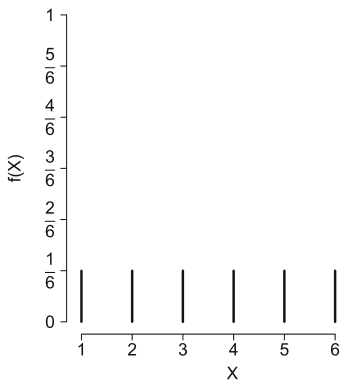
\includegraphics[width=5cm]{content/pdfdiscret.PNG} }}%
\qquad
\subfloat[Fonction de répartition]{{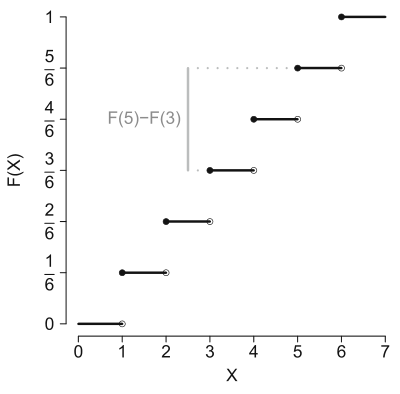
\includegraphics[width=5cm]{content/cdfdiscret.PNG} }}%
\caption{Fonction de densité de probabilité et fonction de répartition pour
le lancer d'un dé dans l'exemple \ref{exemple:4}. «•» se rapporte à une valeur incluse et «$\circ$» à une valeur exclue}%
\label{fig:exemple4}%
\end{figure}

\end{example}

Nous pouvons utiliser la fonction de répartition pour calculer toute probabilité souhaitée, par exemple
$P (X ≤ 5) = F (5) = 5/6$. Ceci est montré sur la figure \ref{fig:exemple4}b où pour $X = 5$, nous obtenons
$F (5) = 5/6$ lors de l'évaluation sur l'axe des $y$. De même, $P (3 <X ≤ 5) = F (5) - F (3) = (5/6) - (3/6) = 2/6$
peut être interprété comme la différence de $F (5)$ et $F ( 3) $ sur l'axe des $y$.





%Here I am talking about a great article \cite{great_article}. And there is also a great conference proceedings \cite{great_proceedings}.

\subsection{Figures}

Here is an example of a figure environment :

\begin{center}
    \begin{figure}[ht!]
        \centering
        
        
\includegraphics[width=5cm, keepaspectratio]{imports/2000.png}
        
        \caption{This is a figure description}
    \end{figure}
\end{center}

\subsection{Item lists}

This is a list of items :

\begin{itemize}
    \item Item 1
    \item Item 2
    \item Item 3
\end{itemize}

\subsection{Footnotes}

This is a footnote \footnote{footnote content}.

\subsection{Tabular}


\begin{center}
    \begin{tabular}{|l|c|r|} % left - center - right
        \hline
        \rowcolor{white!75!black} \textbf{Column 1} & \textbf{Column 2} & \textbf{Column 3} \\
        \hline
        Left aligned lalalalala & centered & Right aligned lalalalala\\
        \hline
         & & \\
        \hline
    \end{tabular}
\end{center}
\fi